\documentclass[addpoints,12pt,answers]{exam}
\usepackage[utf8]{inputenc}
\usepackage{parskip}
\usepackage{color}
\usepackage{graphicx}
\usepackage[normalem]{ulem}
\usepackage{amsmath}
\usepackage{amssymb}
\usepackage{amsfonts}

\definecolor{mycrimson}{cmyk}{0.25,1,.79,.20}
\CorrectChoiceEmphasis{\color{mycrimson}\bfseries}

\title{Lecture Exercise 4: Metal and Phase Diagrams (31 Points)}
\author{Dr. Armen Amirkhanian, P.E.\\CE262--Materials in Civil Engineering}
\date{Due: October 8, 2018}

\begin{document}

\maketitle

\begin{center}
\fbox{\fbox{\parbox{5.5in}{
\vspace{0.1in}
\textbf{By submitting this assignment on Blackboard, you acknowledge that you understand the UA Academic Honor Code. You promise or affirm that you will not at any time be involved with cheating, plagiarism, fabrication or misrepresentation while enrolled as a student at The University of Alabama. You agree that you have read the Academic Honor Code, which explains disciplinary procedures that will result from the aforementioned. You understand that violation of this code will result in penalties as severe as indefinite suspension from the University.
\vspace{0.1in}}}}}
\end{center}



\newpage

\begin{questions}
\question Use the phase diagram below to answer the following questions:
\begin{parts}
\part[5] If I have a combination of 70\% Al$_2$O$_3$--30\% TiO$_2$ at 1600$^\circ$C, how much, percentage-wise, Al$_2$O$_3$ and $\beta$--Al$_2$TiO$_5$ do I form if I hold for $t=\infty$?
\part[1] Does your answer change if I only hold at 1201$^\circ$C?
\part[5] If I have a combination of 5\% Al$_2$O$_3$--95\% TiO$_2$ at 1750$^\circ$C, what are the two phases present and how much, percentage-wise do I have of each if I hold for $t=\infty$?
\end{parts}
\begin{center}
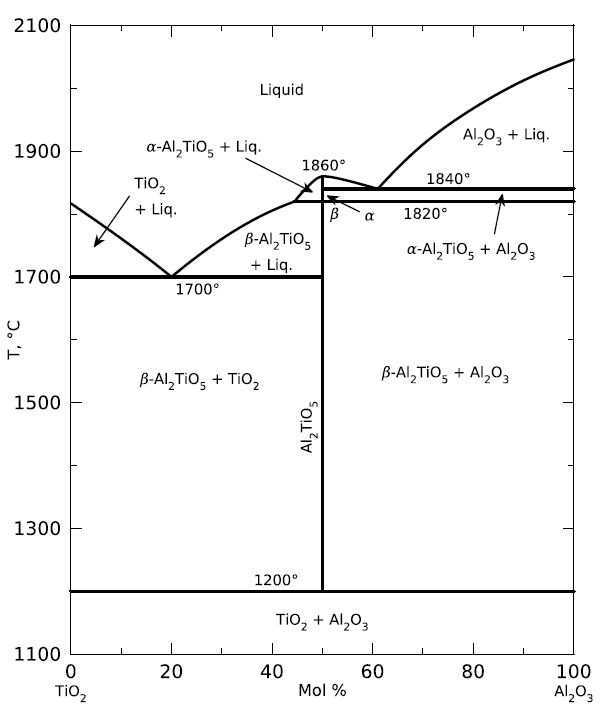
\includegraphics[width=0.7\textwidth]{phasediag.png}
\end{center}

\begin{solution}
The chosen phase diagram is a little unique in that it is split almost perfectly in half. You would not be expected to know this, but the straight line of Al$_2$TiO$_5$ at 50\% means the single phase is congruently melting since the liquid phase has the same composition as the solid phase. Pretty cool (actually, it's pretty hot)!

Anyways, for Part (a), the percentages of phases formed can be calculated via:
\[
\mathrm{\% \beta-Al_2TiO_5}=\dfrac{70-100}{50-100}=60\%
\]

\[
\mathrm{\% Al_2O_3}=\dfrac{70-50}{100-50}=40\%
\]

Part (b) is a type of trick question as the composition from Part (a) does not change between 1201$^\circ$C and 1819$^\circ$C due to the shape of the phase diagram.

Part (c) requires you to estimate where the lever line intersects the liquidus line. The two phases that are present at that composition and temperature are TiO$_2$ and Liquid. The amounts of the two phases are calculated via:
\[
\mathrm{\% TiO_2}=\dfrac{5-12}{0-12}=58\%
\]

\[
\mathrm{\% Liquid}=\dfrac{5-0}{12-0}=42\%
\]
\end{solution}

\question[5] Your time to shine and possibly get a free question on the next exam. Design a 5-answer multiple choice exam question for anything we have covered so far. Indicate the correct answer. Your alternative answers need to be reasonable. Two questions from these submissions will be used on the next exam.

\begin{solution}
This is an open-ended question with all sorts of possible answers. Any reasonable attempt to create a decent question with reasonable alternative answers will receive full credit.
\end{solution}

\newpage
\question[9] This is going to be more of a writing exercise than anything else. Using \textbf{only} three sentences for each microstructure, describe the general process to obtain said microstructure, the general properties of said microstructure, and if said microstructure is desired in civil engineering applications or not:
\begin{itemize}
    \item Pearlite
    \item Bainite
    \item Martensite
\end{itemize}

\begin{solution}\\
\textbf{Pearlite}: Pearlite is typically formed with slower cooling and/or annealing processes at higher temperatures. Pearlitic steels typically have a pearlensence sheen and relatively high strength compared to the other two microstructures. This type of microstructure is desired in civil engineering applications however the cost and production techniques may limit its use.\\

\textbf{Bainite}: Bainite is typically formed with faster cooling and low temperature annealing processes. Bainitic steels are typically harder than pearlitic steels and not as strong. Nevertheless, this type of microstructure can have some applications in civil engineering applications where high-wear is a concern.\\

\textbf{Martensite}: Martensite is typically formed while rapidly cooling a steel. It is generally the hardest microstructure. This type of microstructure can be used in high-wear applications but the high hardness and possibility of brittle fracture generally limits its use in civil engineering applications.
\end{solution}

\question[6] Assuming you have followed ASTM A370, using the 2-inch gauge length specimen shown in Figure 3 in the standard, and the 0.2\% offset yield \textbf{load} for three different samples was 14,000 lb$_f$, 17,000 lb$_f$, and 80,000 lb$_f$, what are the three materials? Assume the minimum specimen thickness as outlined in Note 7 of Figure 3. It is strongly recommended that you use the Knovel material property search as shown in class. Cite your source for each determination. To help guide your selection, your possible choices are listed below:
\begin{itemize}
    \item Rail steel
    \item Aluminum 6061
    \item Stainless Steel 304
    \item Titanium Alloy Grade 5
    \item Tool steel
    \item Poly(methyl methacrylate)
\end{itemize}

\begin{solution}\\
\textbf{14,000 lb$_f$}: This is a yield stress of approximately 45,000 psi which correlates closely to aluminum 6061.\\

\textbf{17,000 lb$_f$}: This is a yield stress of approximately 55,000 psi which correlates closely to rail steel.

\textbf{80,000 lb$_f$}: This is a yield stress of approximately 258,000 psi which correlates closely to tool steel.
\end{solution}

\end{questions}
\begin{center}

\includegraphics[scale=0.6]{88x31.png}\\
This lecture exercise set by Dr. Armen N Amirkhanian is licensed under a Creative Commons Attribution-ShareAlike 4.0 International License.
\end{center}
The Al$_2$O$_3$-TiO$_2$ phase diagram is from the freely available ACerS-NIST Phase Equilibria Diagram database (Version 4.2). The specific citation for the figure is shown below.

Fig. \textbf{92-008}—System TiO$_2$-Al$_2$O$_3$.
P. Pena and S. DeAza, \textit{Ceramica (Florence)}, \textbf{33} [3] 23-30 (1980).

This diagram is a revision of Figs. 316 and 4376 by the current authors, incorporating the later studies of Refs. 1-3:\\

\textbf{1.} R. T. Chudhill; Ph.D. Dissertation. University of Sheffield, Sheffield, United Kingdom, 1965.\\

\textbf{2.} J. A. Imlach and F. P. Glasser, \textit{Trans. Br. Ceram. Soc.}, \textbf{67} [12] 581-609 (1968).\\

\textbf{3.} J. S. Moya Corral and A. Garcia Verduch, \textit{La Ceramica}, \textbf{30} [4] 19-22 (1977).\\



\end{document}